%%%%%%%%%%%%%%%%%%%%%%%%%%%%%%%%%%%%%%%%%%%%%%%%%%%%%%%%%%%%%%%%%%%%%%%%%%%%%%%%%
% Diseño
%%%%%%%%%%%%%%%%%%%%%%%%%%%%%%%%%%%%%%%%%%%%%%%%%%%%%%%%%%%%%%%%%%%%%%%%%%%%%%%%%

\chapter{Diseño de la propuesta} % (fold)
\label{cha:Diseno}

    %% Aquí hay que detallar y justificar las decisiones que se tomen (hacer varias propuestas pero desarrollar solo la
    %% mejor) (siempre es bueno una tabla comparativa con pros y contras o ticks)

    \section{Tecnologías empleadas} % (fold)
    \label{sec:TecnologiasEmpleadas}

        \subsection{C} % (fold)
        \label{sub:CLanguage}
        
            El lenguaje utilizado para la mayor parte del proyecto ha sido C. C es un lenguaje desarrollado en 1972 por
            Dennis Ritchie en los Laboratios Bell. Fue creado para la creación de sistemas operativos, como UNIX, y es
            muy valorado por su eficiencia.

            En la actualidad, es uno de los lenguajes más populares. Está disponible en muchas plataformas, desde
            superordenadores, hasta sistemas empotrados. Fue diseñado para mapear las instrucciones escritas en C a
            lenguaje máquina de forma muy eficiente, con pocas instrucciones, esto hace que sea muy eficiente en
            cualquier plataforma en la que se utilice.\cite{wikipedia_c_language}

            Es por esta eficiencia, por la que se ha utilizado en el proyecto. Cualquier instrumento musical, y en
            especial una batería, requiere que las acciones realizadas por el músico tengan una reacción rápida por el
            sistema, y C puede proporcionar esta velocidad.

        % subsection C (end)

        \subsection{Visual Studio Code} % (fold)
        \label{sub:VisualStudioCode}

            Visual Studio Code es un editor de texto diseñado por Microsoft para Windows, Linux y macOS, lanzado al
            público en 2016.

            Su sencillez, compatibilidad con una gran cantidad de lenguajes de programación y una extensa biblioteca de
            extensiones han hecho que VS Code sea uno de los editores de texto más populares entre los programadores.
            \cite{wikipedia_vs_code}

            \begin{figure}[ht]
                \centering
                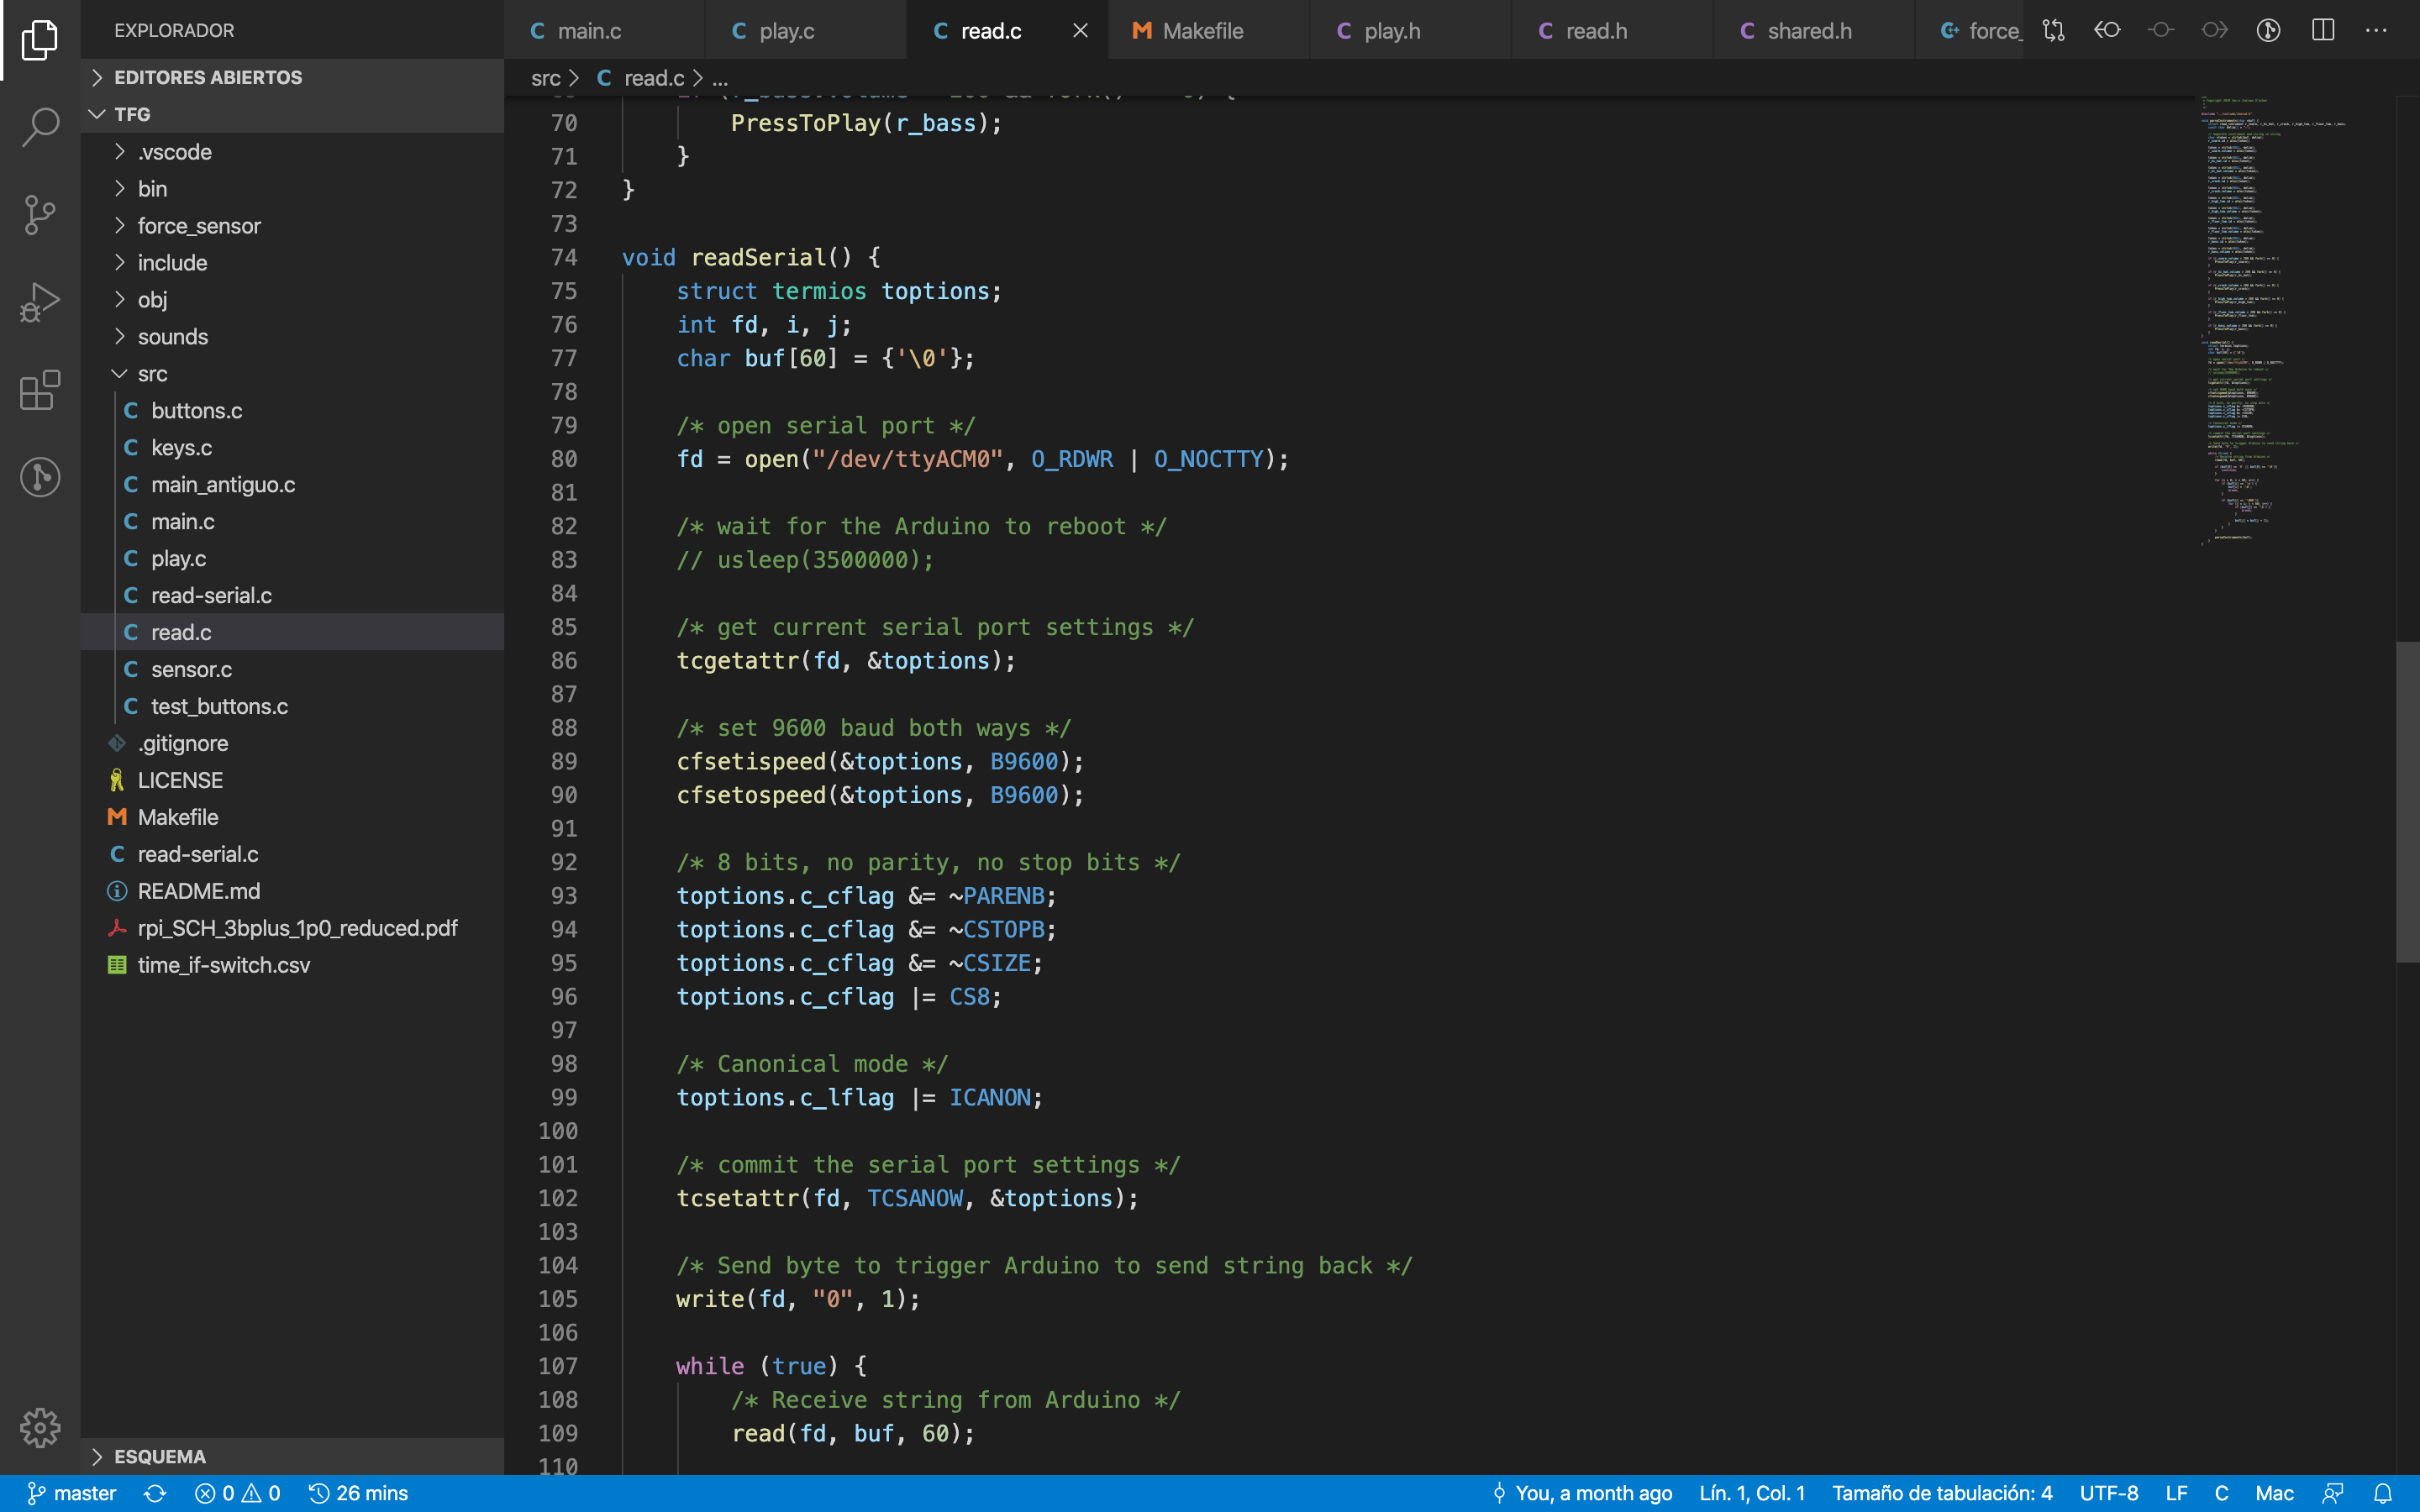
\includegraphics[width=\textwidth]{vs_code}
                \caption{Captura de pantalla de Visual Studio Code \label{fig:VisualStudioCode}}
            \end{figure}
            
            \newpage
        
        % subsection Visual Studio Code (end)

        \subsection{Github} % (fold)
        \label{sub:Github}

            Github es un servicio de alojamiento de código abierto y control de versiones mediante Git.

            En este proyecto se ha utilizado principalmente para llevar ese control de versiones del código y para
            organizar los diferentes pasos a dar y los errores encontrados durante el desarrollo mediante su capacidad
            de crear \textit{issue}. Aparte, Github permite que este código esté disponible para el acceso de cualquier
            persona y que cualquiera pueda contribuir a él.

            \begin{figure}[ht]
                \centering
                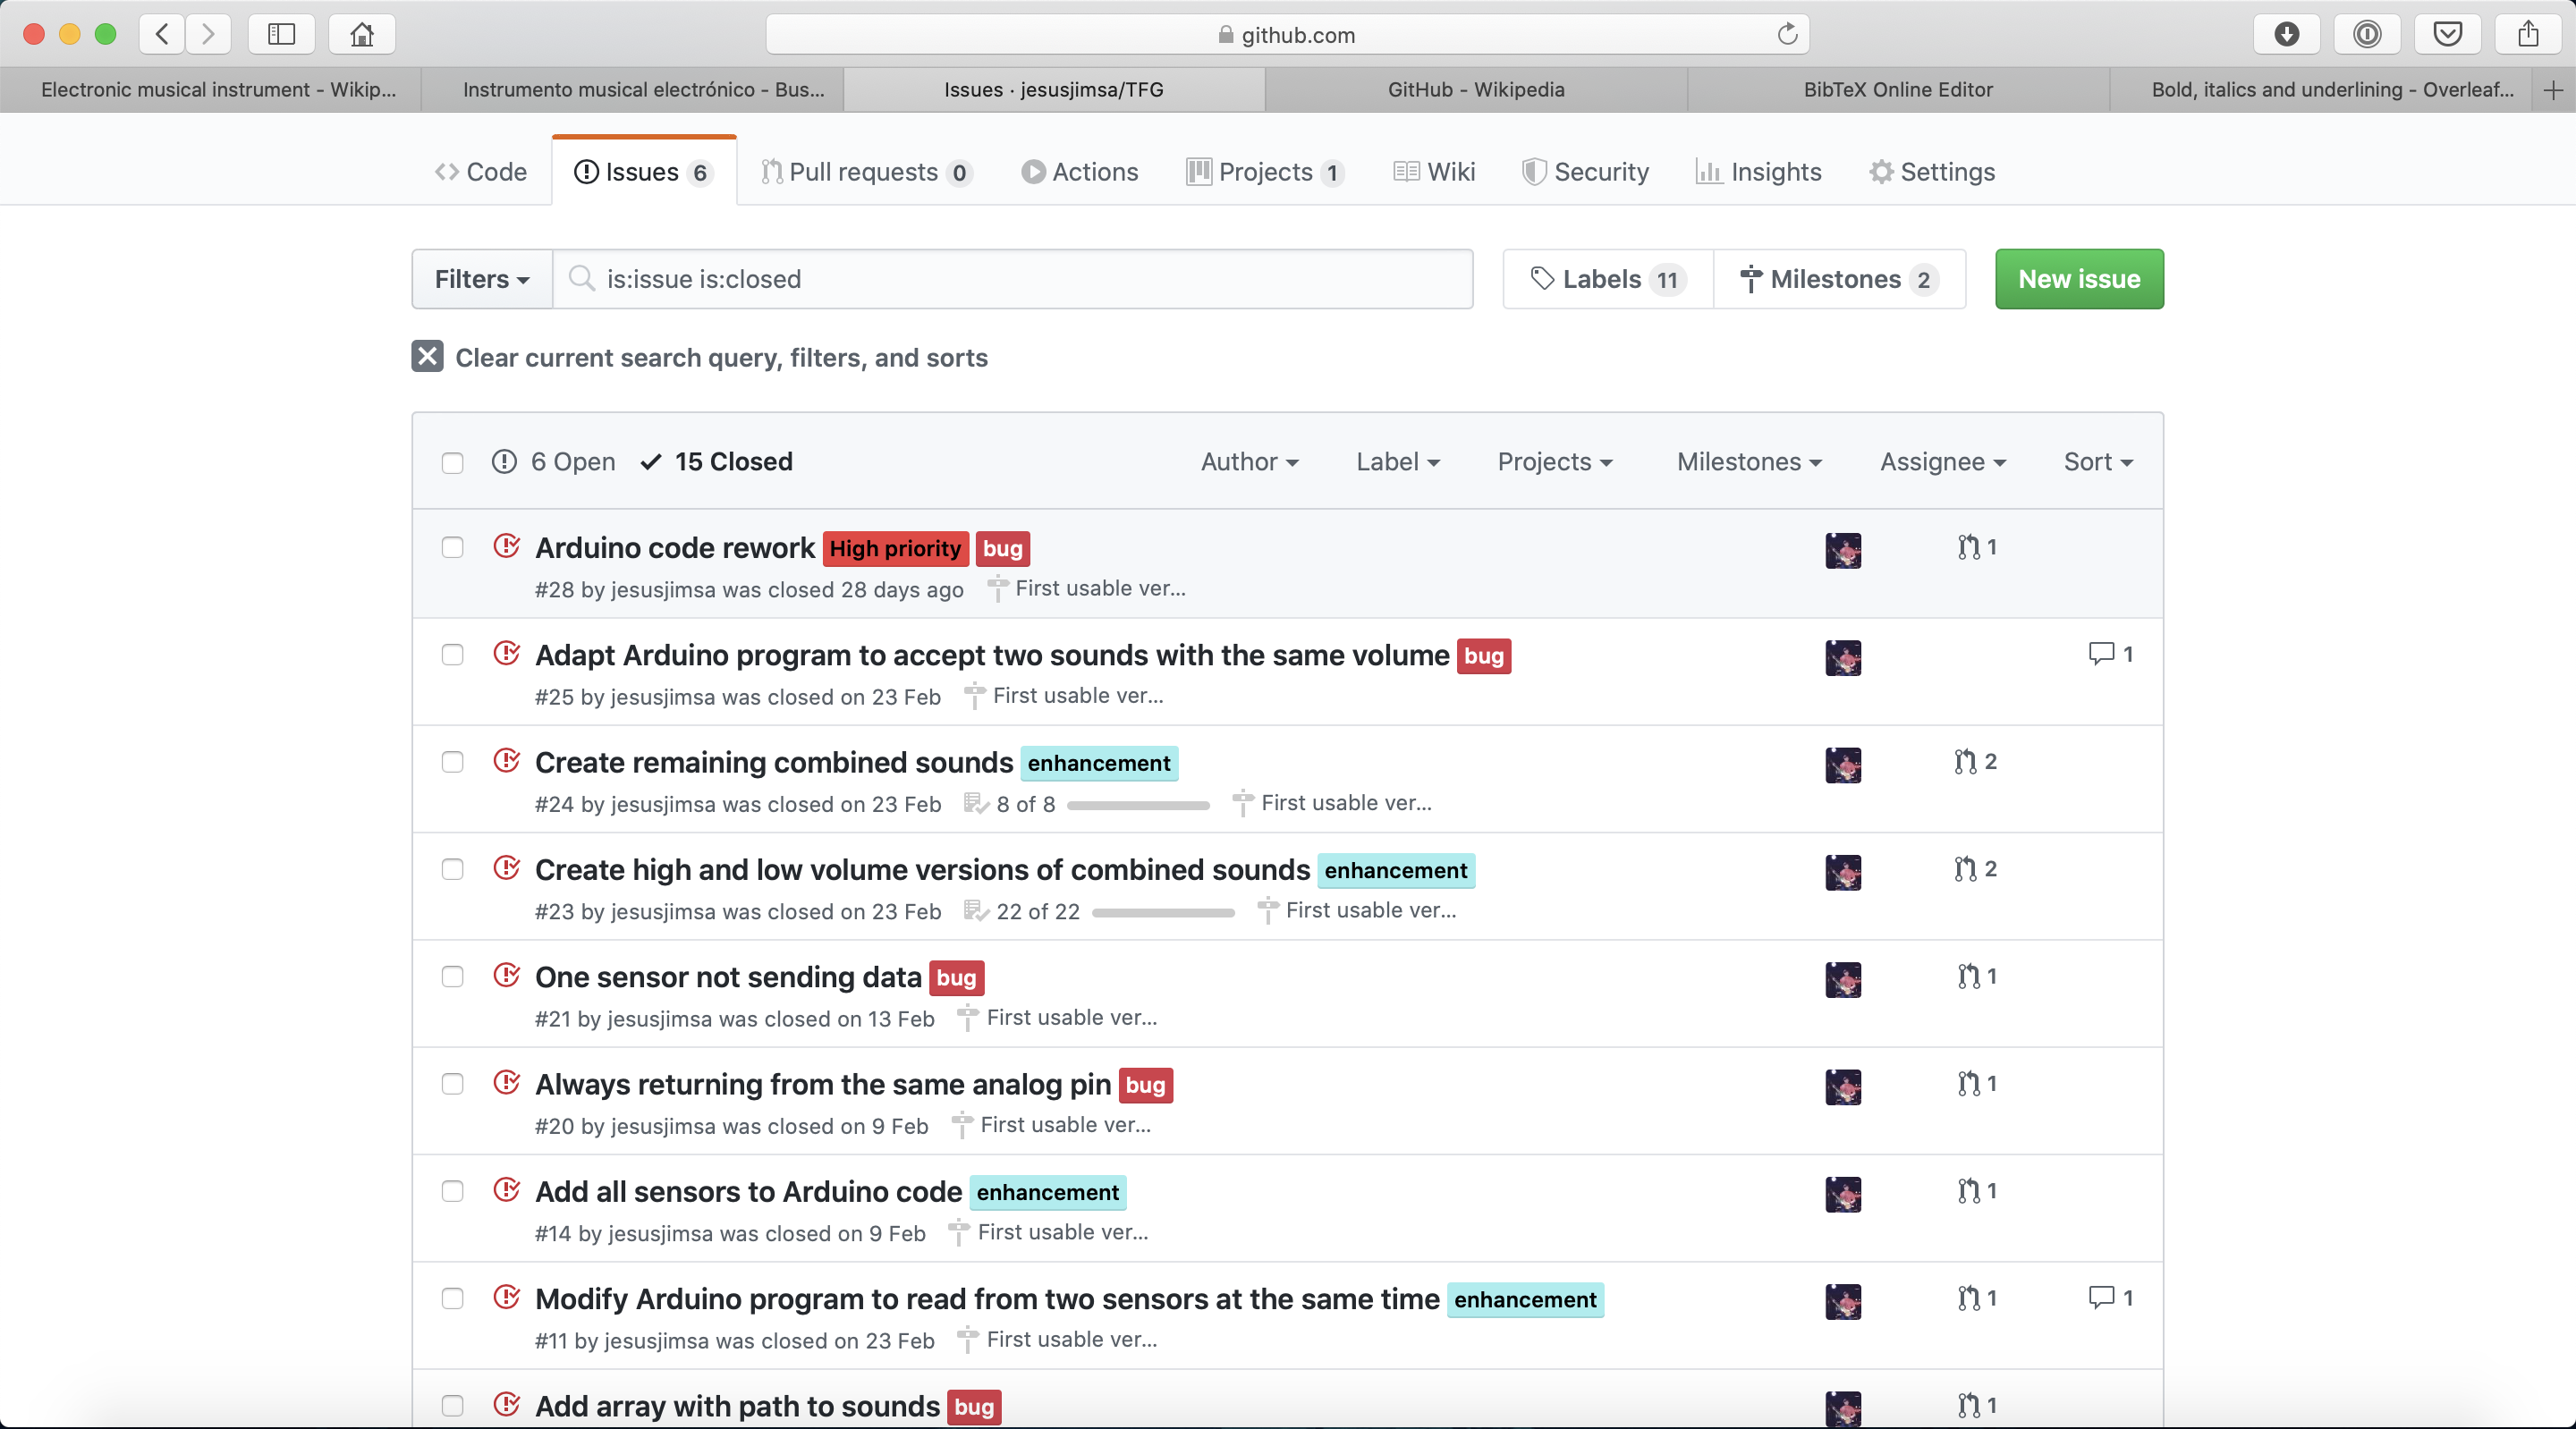
\includegraphics[width=\textwidth]{github_issues}
                \caption{Captura de pantalla de las issues de Github del proyecto \label{fig:GithubIssues}}
            \end{figure}
            
            \newpage
        
        % subsection Github (end)

        \subsection{Clockify} % (fold)
        \label{sub:Clockify}

            Clockify es una aplicación de seguimiento de tiempo. Ha sido utilizada para llevar un seguimiento de cuánto
            tiempo ha sido dedicado a la creación y desarrollo de este proyecto y su memoria.

            \begin{figure}[ht]
                \centering
                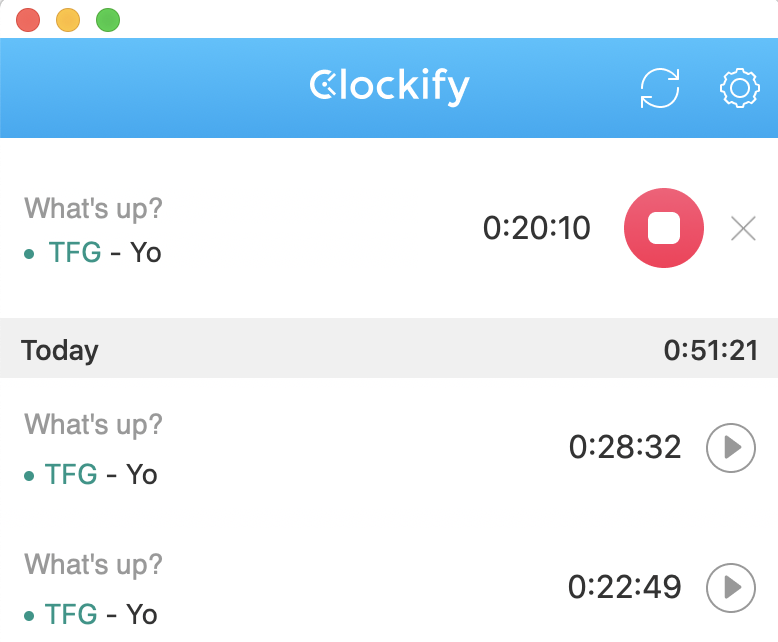
\includegraphics[width=\textwidth/2]{clockify}
                \caption{Captura de pantalla de Clockify \label{fig:ClockifyCaptura}}
            \end{figure}
        
        % subsection Clockify (end)

        \subsection{Overleaf} % (fold)
        \label{sub:Overleaf}

            Overleaf es un editor de LaTeX online y colaborativo. Permite crear documentos en LaTeX y la colaboración de
            hasta dos personas en su modalidad gratuita.

            En este proyecto, ha facilitado la compartición de esta memoria entre alumno y tutor para su corrección, a
            parte de servir como editor principal de LaTeX.

            \begin{figure}[ht]
                \centering
                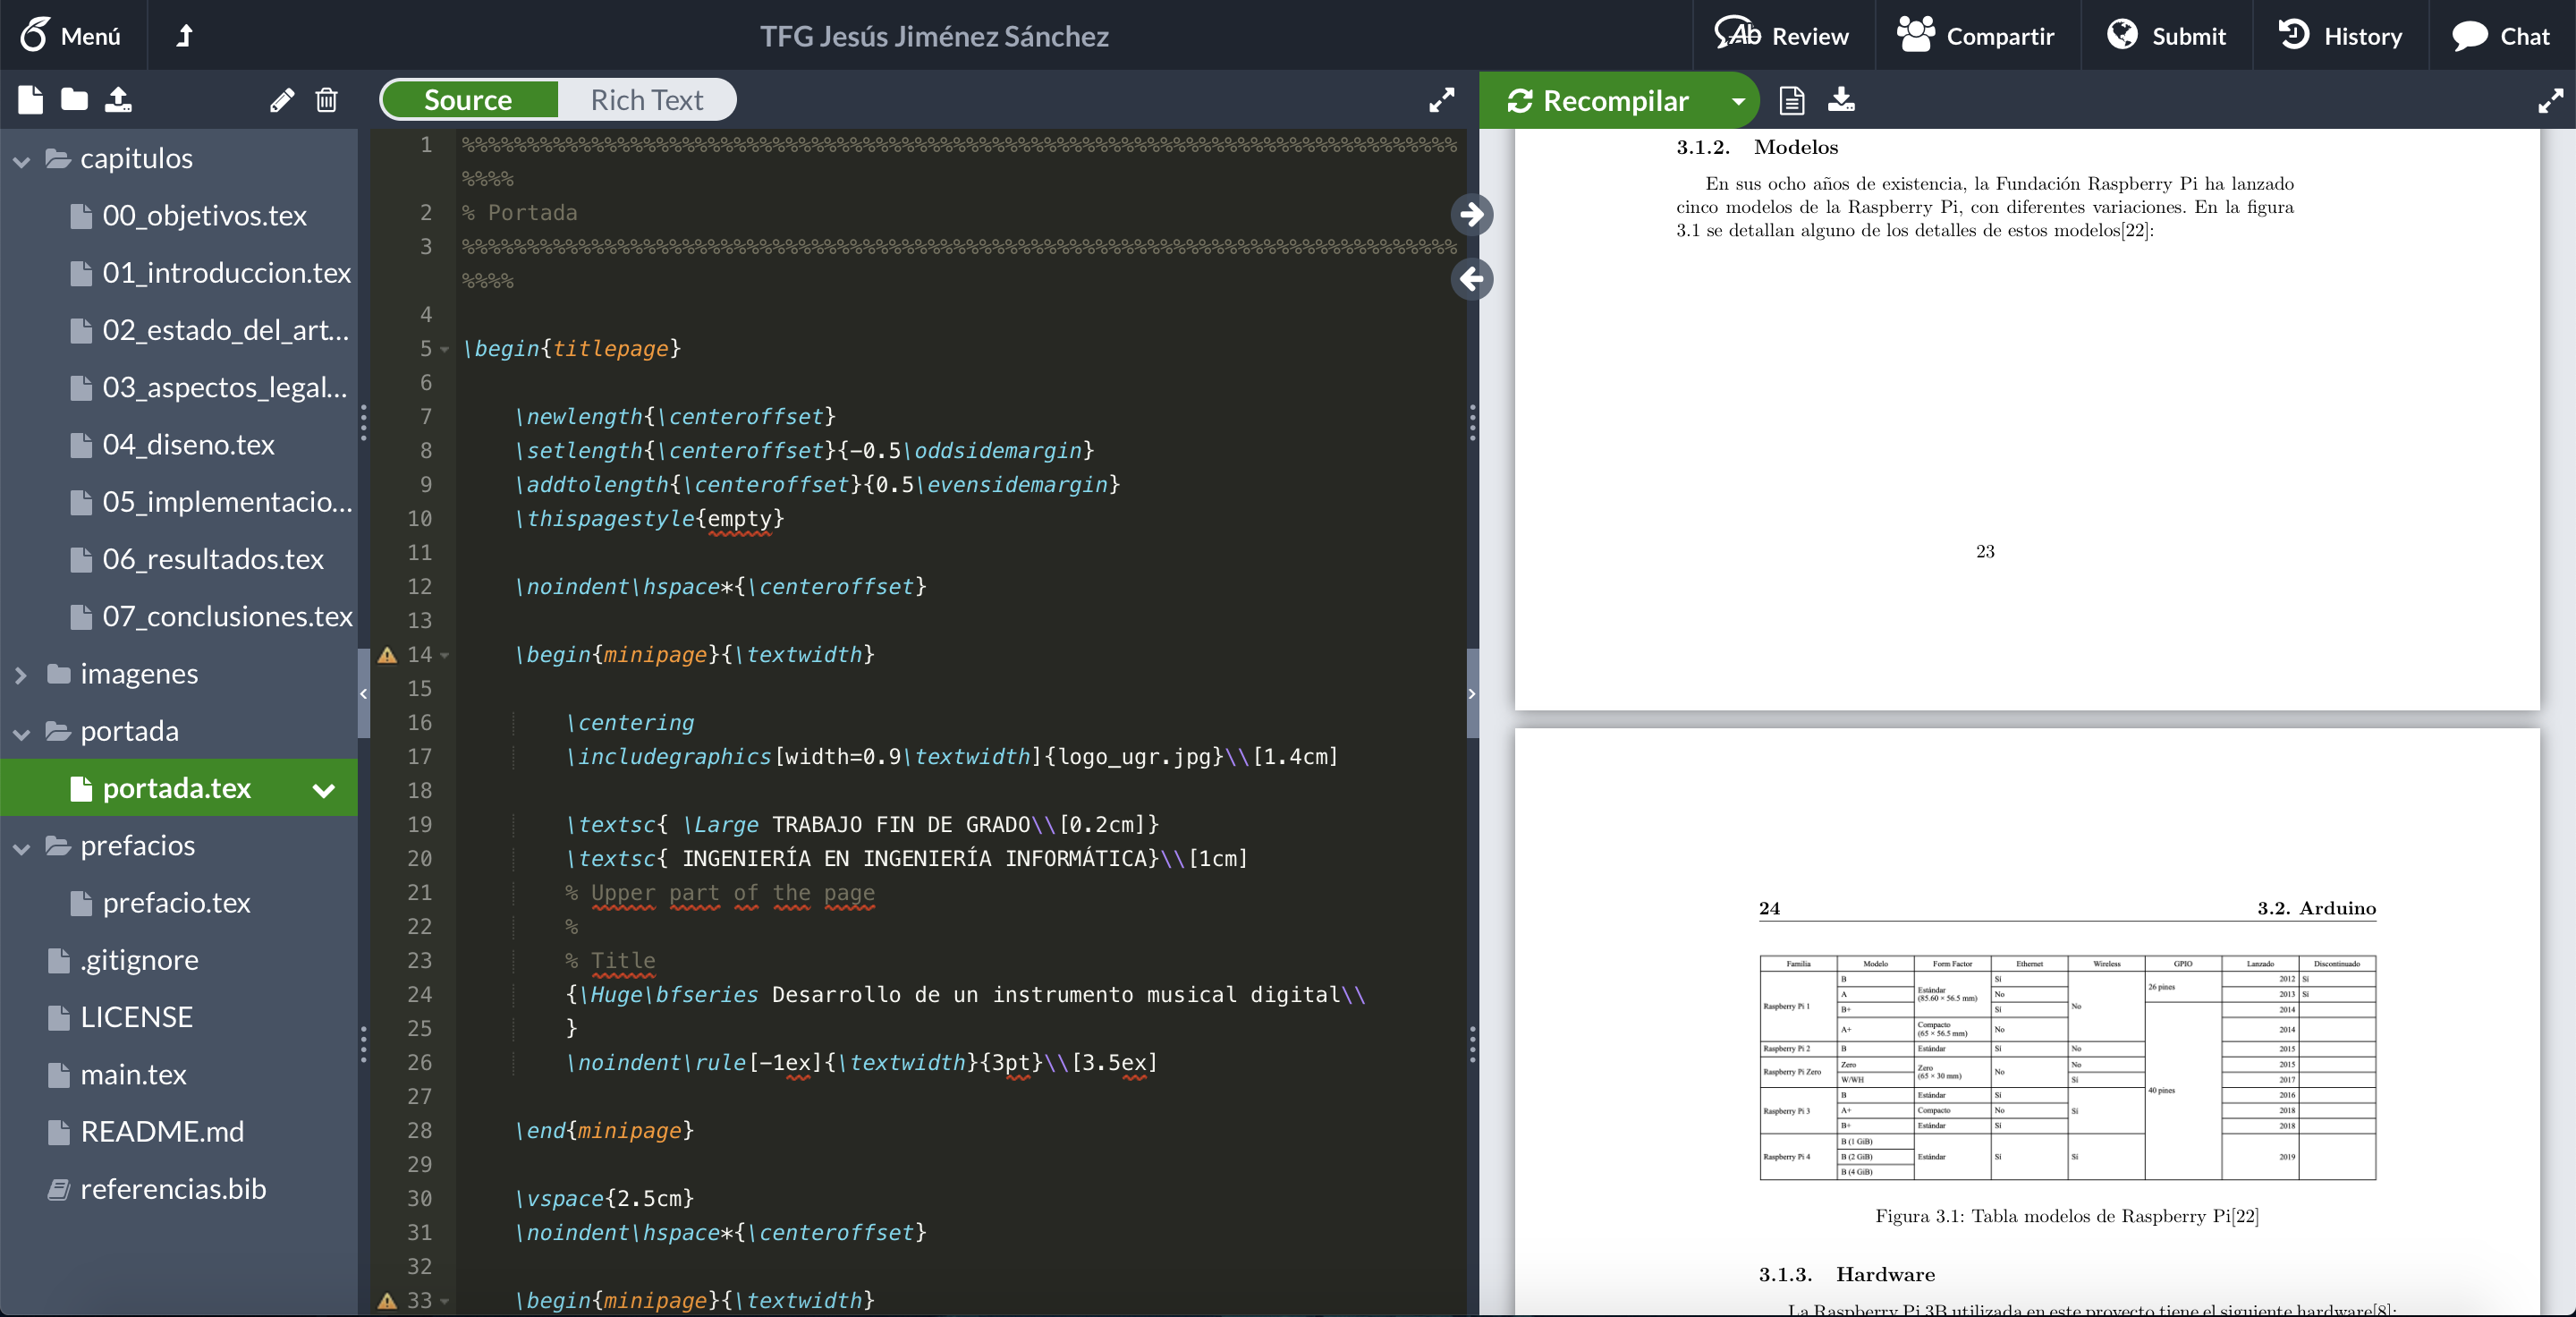
\includegraphics[width=\textwidth]{captura_overleaf}
                \caption{Captura de pantalla de Overleaf \label{fig:OverleafCaptura}}
            \end{figure}
        
        % subsection Overleaf (end)

    % section Tecnologías empleadas (end)

    \section{Decisiones tomadas} % (fold)
    \label{sec:DecisionesTomadas}

        La primera decisión fue entre hacer detección binaria de la entrada, es decir, si el parche ha sido golpeado o
        no, y hacer que estas entradas sean concurrentes (al golpear dos parches, el sonido de ambos suena al mismo
        tiempo), o hacer detección de distintos sonidos en un mismo parche, dependiendo de cómo se golpee el parche (en
        el centro, en el lateral, con más o menos fuerza…) el sonido emitido es diferente.\newline

        Se decide empezar con la primera alternativa y dejar la segunda para más adelante, en caso de tener tiempo.

        \subsection{Librería de reproducción de sonido ¿?} % (fold)
        \label{sub:LibreriaDeReproduccionDeSonido}

            \begin{itemize}
                \item
                playsound\cite{playsound}: Al principio se comenzó buscando implementar el proyecto en Python, por ser
                un lenguaje sencillo y con gran variedad de librerías. Sin embargo, tras probar playsound, la librería
                de reproducción de sonidos más popular de Python, se decidió que era muy lenta, y en este proyecto, la
                velocidad a la que se reproducen los sonidos es primordial. Por esta razón, se descarta playsound.
                \item
                mpg123\cite{mpg123}: Librería y programa en C más rápido que playsound de Python. Tiene el problema de
                hacer que haya fallos de memoria cuando se usan hebras para reproducir varios sonidos al mismo tiempo,
                pero se soluciona utilizando procesos en su lugar.
            \end{itemize}

        % subsection Librería de reproducción de sonido (end)

        \subsection{Otras librerías} % (fold)
        \label{sub:OtrasLibrerias}

            \begin{itemize}
                \item
                Wiring Pi\cite{wiringPi}: Para realizar la conexión de sensores y botones a la Raspberry Pi se utiliza
                la librería wiringPi, que es la estándar en este tema.
            \end{itemize}

        % subsection Otras librerías (end)

        \subsection{if-else vs switch} % (fold)
        \label{sub:if-else_vs_switch}

            Al pulsar una tecla, el número leído se envía a una función que selecciona qué sonido hay que reproducir en
            ese momento, dependiendo de qué sonido corresponda a ese número. Este proceso de selección se puede hacer
            con una estructura de \textit{if-else} anidados o con un \textit{switch-case}.\newline

            Para decidir cuál de las dos soluciones se implementa en la versión final se realizó un test en el que cada
            vez se ejecutan más iteraciones del programa cambiando de sonido en cada una de ellas. Se empieza con 1
            iteración y se termina con 10000000 iteraciones.\newline

            \begin{figure}[ht]
                \centering
                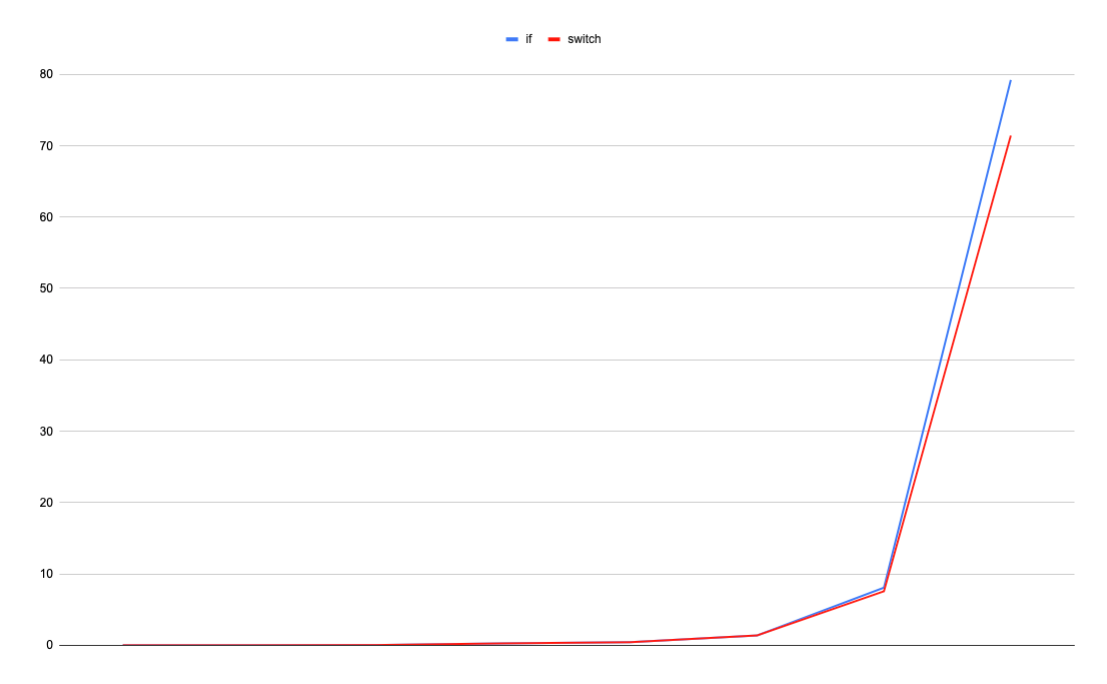
\includegraphics[width=\textwidth]{grafica_if_switch}
                \caption{Gráfica comparativa if-else vs switch \label{fig:GraficaIfVsSwitch}}
            \end{figure}

            \begin{center}
                \begin{tabular}{ |c|c|c| }
                    \hline
                        iterations & if & switch \\
                        \hline\hline
                        1 & 0.000243 & 0.000270 \\
                        \hline
                        10 & 0.002797 & 0.002485 \\
                        \hline
                        100 & 0.027775 & 0.027261 \\
                        \hline
                        1000 & 0.260075 & 0.261464 \\
                        \hline
                        10000 & 0.431544 & 0.425668 \\
                        \hline
                        100000 & 1.368561 & 1.374575 \\
                        \hline
                        1000000 & 8.070825 & 7.560718 \\
                        \hline
                        10000000 & 79.199539 & 71.409653 \\
                    \hline
                \end{tabular}
            \end{center}

            Como se puede ver en la figura \ref{fig:GraficaIfVsSwitch}, la diferencia no es apreciable hasta las
            1000000 iteraciones, pero después pasa a casi 8 segundos de diferencia en 10000000 iteraciones. Por
            esta razón se ha decidido que la función utilice la estructura \textit{switch-case}.\newline

            Finalmente, debido a la manera en la que realizan las comprobaciones de qué botones y sensores son
            utilizados, aunque un \textit{switch-case} es más rápido, esta estructura se reserva para la versión del
            programa que reproduce los sonidos leyendo del teclado. En el programa que controla los sensores se
            utiliza una estructura \textit{if-else}.

        % subsection if-else vs switch (end)

    % section Decisiones tomadas (end)

    \section{Arduino vs Raspberry Pi} % (fold)
    \label{sec:ArduinoVsRaspberryPi}

        Para la recepción de las señales del sensor de presión RP c18.3, se plantean dos opciones, se puede utilizar
        la propia Raspberry Pi en la que se ejecuta el programa que maneja los sonidos o una Arduino Nano. En el
        proyecto resultante se utiliza finalmente la Arduino debido a dos razones principales.\newline

        La primera razón es el precio y la escalabilidad, una Raspberry Pi cuesta 39,95\euro{} mientras que una
        Arduino Nano cuesta 10\euro{}. Una Arduino Nano cuenta con menos pines de E/S, pero añadir una placa es más
        barato y sencillo que añadir una placa de Raspberry Pi.\newline

        La segunda razón es la implementación del programa que se encarga de el sensor de presión. En Internet se
        pueden encontrar ejemplos y tutoriales refiriéndose a cómo implementar el sistema en una Arduino, pero no
        es tan fácil encontrar información para hacerlo desde una Raspberry Pi.\newline

        Por estas razones se elige realizar la recepción de las señales del sensor de presión desde la Arduino,
        haciendo el proceso más sencillo y más barato.

        \subsection{Conexión} % (fold)
        \label{sub:Conexion}

            Para realizar la conexión de los sensores se utilizan cables de protoboard conectados de la forma
            explicada en la figura \ref{fig:EsquemaConexion}:

            \begin{figure}[ht]
                \centering
                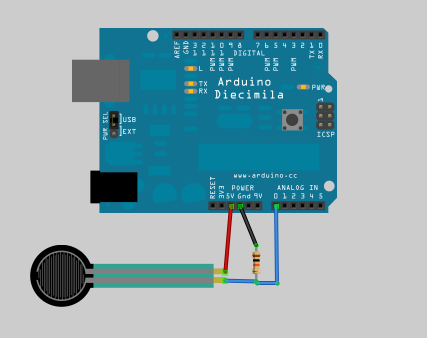
\includegraphics[width=\textwidth]{force_sensor_arduino}
                \caption{Esquema de conexión de sensores de presión\cite{force_sensor_arduino}
                         \label{fig:EsquemaConexion}}
            \end{figure}
        
        % subsection Conexión (end)

    % section Arduino vs Raspberry Pi (end)

% chapter Diseño (end)